\section{Einleitung}
\sectionauthor{Natalie Teplitska, Leo Bergmann}

Unser Kurs beschäftigte sich mit der computergestützten Gewinnung von Bildern aus Rohdaten. Bei vielen Untersuchungsobjekten in der Physik und Medizin benötigt man bildgebende Verfahren, weil Messungen nur indirekt möglich sind. Daher erarbeiteten wir uns notwendige mathematische Konzepte der Informationstheorie (IT) und wandten diese auf ein Beispiel aus der Radioastronomie und auf Computertomografie an.

Da wir Theorien aus diversen Anwendungsbereichen benötigten, haben wir uns diese bereits vor der Akademie im mithilfe vom Postern angeeignet und innerhalb der ersten Tage den anderen vorgestellt. Dazu hielt jede*r einen 15 Minuten Vortrag auf Grundlage des Posters innerhalb eines durchdachten Rotationssystems. Die Poster wurden am ersten Tag aufgehängt und weckten somit das Interesse der anderen Kurse und personalisierten den Standort.

Diese Fülle an Informationen vervollständigten Gordian und Philipp mit ihrem Wissen und ihrer Erfahrung in mehreren Input-Sessions, welche vornehmlich die erste Woche in Anspruch nahmen. Wir erhielten, alternierend von Gordian und Philipp eine Einführung in die IT, Radioastronomie, Staubtomografie und ganz viel Mathe.

\begin{figure}
    \centering
    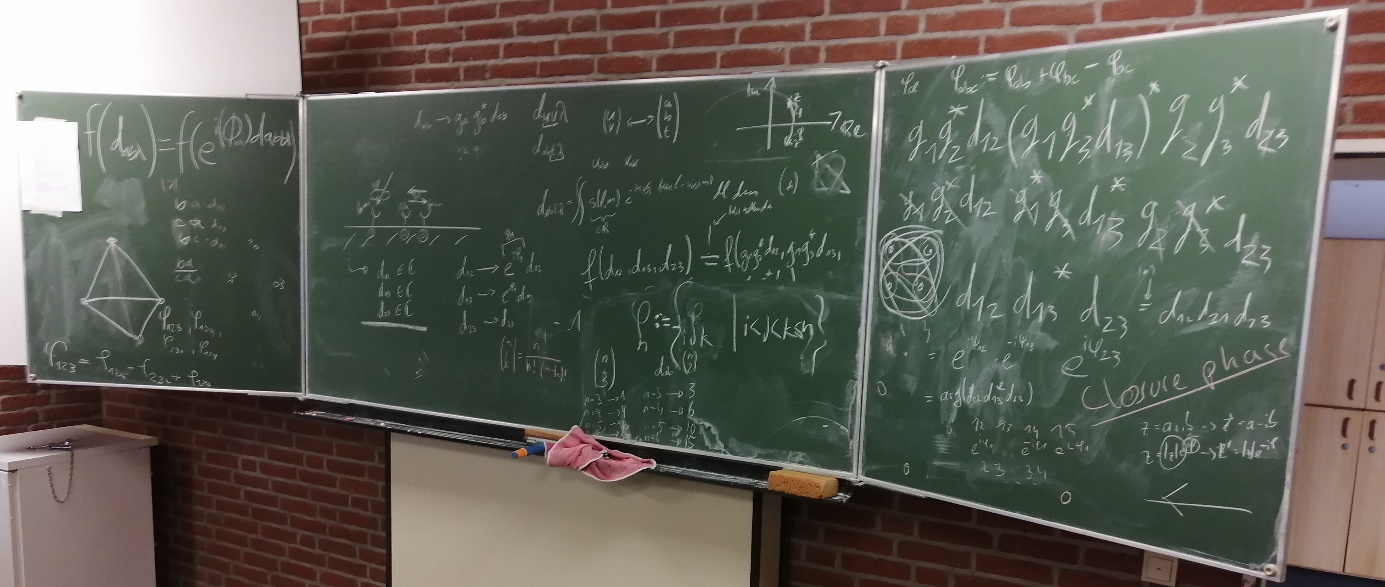
\includegraphics{k4.2/tafelbild.png}
    \caption{Tafel-Chaos}
\end{figure}

\begin{figure}
    \centering
	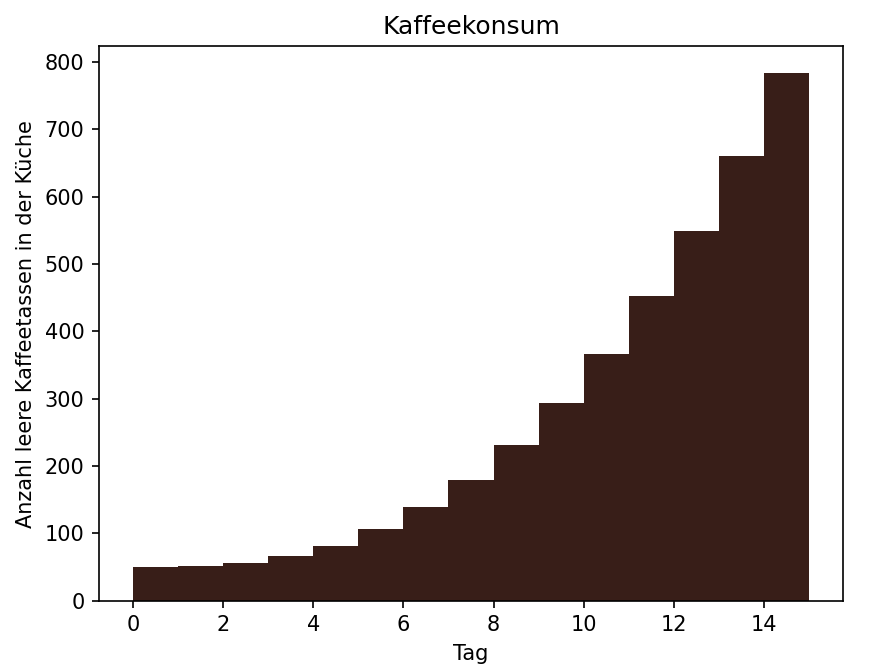
\includegraphics[width=0.5\textwidth]{k4.2/kaffee.png}
	\caption{Kaffeekonsum}
    \label{k4.2.fig.kaffee}
\end{figure}

In der zweiten Woche arbeiteten wir an eigenen Projekten. Je zwei Projektteams beschäftigen sich mit Datenverarbeitung aus der Radioastronomie und der Computer-Tomographie. Das fünfte Projektteam erarbeitete weitere mathematische Konzepte, welche für beide Projekte essenziell waren. Die Projektarbeit gab uns die Möglichkeit, unser Wissen eigenständig anzuwenden. Allerdings mussten besonders gegen Ende der Akademie Teile der Projektarbeit außerhalb der Kurse erledigt werden, was sich im allgemeinen Kaffeekonsum der Akademie niederschlug (siehe \cref{k4.2.fig.kaffee}).
Es war ein hartes Stück Arbeit, welches wir mit Python und viel Kaffee jedoch schlussendlich in den Griff bekamen. Und das Ergebnis kann sich in jedem Fall sehen lassen.
